%! suppress = MissingLabel

В этой главе собраны некоторые общие знания о типах.

Разделы~\ref{subsec:variance}, ~\ref{subsec:isomorphism} в основном следуют~\cite[глава 1]{maguire-types}.

\subsection{Вариантность} \label{subsec:variance}

В этом параграфе мы будем рассматривать тему с точки зрения программирования~\cite[глава 3]{maguire-types}, не отдавая должного теории категорий.
Восполнить пробел можно с помощью замечательной статьи, написанной в жанре пьесы~\cite{hinze2012functional}.

\vocab{Ковариантный функтор} --- пара из некоторого типового конструктора \texttt{F} и операции на функциях \texttt{fmap :: (a -> b) -> (F a -> F b)}.
Плюс законы о том, что \texttt{fmap} уважает \texttt{id} и композицию.

\begin{minted}{haskell}
    class Functor f where
      fmap :: (a -> b) -> (f a -> f b)
\end{minted}

\begin{figure}[H]
    \centering
    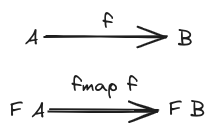
\includegraphics[width=0.3\textwidth]{figs/functor}
\end{figure}

\vocab{Контравариантный функтор} --- пара из типового конструктора и операции на функциях, разворачивающей стрелку.
Плюс соответствующие законы.

\begin{minted}{haskell}
    class Contravariant f where
      contramap :: (a -> b) -> (f b -> f a)
\end{minted}

\begin{figure}[H]
    \centering
    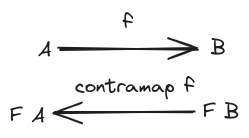
\includegraphics[width=0.3\textwidth]{figs/contra-functor}
\end{figure}

Типовой конструктор можно объявить ковариантным или контравариантным функтором (или никаким из них) относительно некоторого типового параметра в зависимости от вида декларации соответствующих конструкторов данных.
А именно, от знака позиций, в которых входит этот типовой параметр в тип.

Разовьём интуитивное понимание знаков позиций.
Тип \mintinline{haskell}{A} входит в положительной позиции в \mintinline{haskell}{B} если его значение можно извлечь из \mintinline{haskell}{B}.
И наоборот, тип \mintinline{haskell}{A} входит в отрицательной позиции, если его значение нужно, наоборот, предоставить.
Рассмотрим знаки позиций типов в базовых типовых конструкторах:
\begin{center}
    \begin{tabular}[h]{|c|c|c|}
        \hline
        Тип                              & знак позиции \mintinline{haskell}{A} & знак позиции \mintinline{haskell}{B} \\
        \hline
        \mintinline{haskell}{Either A B} & $+$                                  & $+$                                  \\
        \mintinline{haskell}{(A, B)}     & $+$                                  & $+$                                  \\
        \mintinline{haskell}{A -> B}     & $-$                                  & $+$                                  \\
        \hline
    \end{tabular}
\end{center}

Действительно, из суммы и произведения можно извлечь компоненты с помощью паттерн-матчинга, а из стрелки можно получить правый тип апплицируя её к аргументу.
В то же время значение типа слева от стрелки нужно предоставить.

На плюс и минус действуют интуитивные алгебраические законы при рассмотрении более сложных типов.
Рассмотрим на примере \mintinline{haskell}{f :: ((A, B) -> C) -> (D, E)}.
\begin{itemize}
    \item Плюс на плюс даёт плюс.
    Действительно, нужно лишь применить две элиминации вместо одной, чтобы получить заветный тип.
    В нашем примере, чтобы получить \mintinline{haskell}{D}, нужно сначала апплицировать функцию, а потом разобрать пару.
    \item Плюс на минус (и наоборот) даёт минус.
    Действительно, \mintinline{haskell}{C} нам нужно предоставить: \mintinline{haskell}{f (\ab -> provideC)}.
    \item Минус на минус даёт плюс.
    Пару \mintinline{haskell}{(A, B)} нам предоставляют: \mintinline{haskell}{f (\ab -> ...)}.
\end{itemize}

\begin{task}
    Убедитесь что плюс на минус даёт минус.
\end{task}

Возвращаясь к функторам, если типовой параметр входит в декларацию только в положительных позициях, типовой конструктор можно объявить ковариантным функтором относительно этого параметра.
Если в только в отрицательных~--- контравариантным функтором.
Если в обоих, то никаким функтором объявить нельзя.
Соответственно, будем называть типовые параметры ковариантными, контравариантными и инвариантными.

\begin{task}
    Объявите \mintinline{haskell}{instance Contravariant F} для \mintinline{haskell}{data F a = L (a -> ()) | R Int}.
\end{task}

Таким образом, можно понимать ковариантный функтор как вычисление, результат которого можно пост-обработать, а контравариантный функтор --- как вычисление, аргументы которого можно пред-обработать.

Тип от двух положительных параметров можно объявить \vocab{бифунктором}:
\begin{minted}{haskell}
    class Bifunctor f where
      bimap :: (a -> c) -> (b -> d) -> f a b -> f c d
\end{minted}

Тип от двух параметров, положительного и отрицательного, --- \vocab{профунктором}:
\begin{minted}{haskell}
    class Profunctor p where
      dimap :: (c -> a) -> (b -> d) -> p a b -> p c d
\end{minted}

Профункторы являются некоторыми обобщениями функциональной стрелки.
Например, если у нас есть SQL запрос, который по данным возвращает результат, его можно объявить профунктором с семантикой --- добавить пред-обработку входных данных и пост-обработку выходных:
\begin{minted}{haskell}
    dimap serialize deserialize (query :: Sql Text Text) :: Sql Age [User]
\end{minted}

Также понятие вариантности часто встречается в объектно ориентированных языках (да и вообще в теории подтипизации) для обозначения возможности дополнить отношение подтипизации на полиморфные типы.

Действительно, \vocab{отношение подтипизации} \texttt{B <: A} говорит о том, что значение типа \texttt{B} безопасно использовать в позиции, где ожидается значение типа \texttt{A}.
Иначе говоря, существует функция \texttt{upcast :: B -> A}.
Если типовой конструктор \texttt{F a} ковариантен относительно параметра \texttt{a}, то по \texttt{upcast} найдётся \texttt{upcast' :: F B -> F A}.
То есть отношение подтипизации также автоматически включает \texttt{F B <: F A}.
Контравариантный случай аналогично.

\begin{task}
    Убедитесь в вашем любимом языке с поддержкой вариантности, что минус на минус даёт плюс.
\end{task}

\subsection{Изоморфизм} \label{subsec:isomorphism}

Пусть нам нужно спроектировать функцию или модель данных.
Мы начинаем с декларации типа, как её выбрать и из каких вариантов?
Для начала поймём, когда два типа взаимозаменимы, для этого рассмотрим понятия изоморфизма.

Два типа \texttt{A} и \texttt{B} называются \vocab{изоморфными} (обозначают \texttt{A $\iso$ B}) тогда и только тогда, когда существует такая пара функций \texttt{to :: A -> B} и \texttt{from :: B -> A}, что\footnote{Под равенством термов можно понимать разное, например, $\alpha\beta\gamma$-эквивалентность. Мы будем пользоваться \vocab{экстенсиональным равенством} для функций~--- две функции равны, когда равны их результаты на всех входах. \url{https://ncatlab.org/nlab/show/function+extensionality}}
\begin{minted}{c}
    to . from = id
    from . to = id
\end{minted}

Иначе говоря, между обитателями таких типов можно установить взаимно-однозначное соответствие.
Легко понять, что со смысловой точки зрения не принципиально, какой из изоморфных типов использовать --- их можно заменять друг на друга, добавляя вызовы функций перехода.
Такие два типа заключают в себе одинаковое ``количество информации''.
Например, типы \mintinline{haskell}|Bool| и \mintinline{haskell}|Maybe ()| в этом смысле совершенно взаимозаменимы.
Покажем это, предъявив пару взаимообратных функций\footnote{Нужно не забыть показать взаимообратность функций, но это делается тривиально перебором входов (может быть с помощью индукции) и редукцией.}:
\begin{minted}{haskell}
    to :: Bool -> Maybe ()
    to b = if b then Just () else Nothing

    from :: Maybe () -> Bool
    from m = case m of Nothing -> False; Just () -> True
\end{minted}

Несмотря на смысловую взаимозаменимость, для кодирования информации о том, передал ли пользователь программе определённый флаг, мы, скорее всего, воспользуемся типом \mintinline{haskell}|Bool| ввиду нефункциональных соображений о читабельности кода.
Аналогично можно рассматривать соображения эффективности.

С категорным взглядом на происходящее можно ознакомиться в~\cite{hinze2010reason}.
Мы же придерживаемся теоретико-множественной интерпретации типов.

\subsubsection{Кардинальность: суммы, произведения, экспоненты} \label{subsubsec:cardinality}

Типы можно воспринимать как синтаксис для записи множеств, а населяющие их термы~--- как синтаксические записи элементов этих множеств.
Так терм \mintinline{haskell}|(True, False)|~--- запись элемента множества пар, записываемого в синтаксисе типов как \mintinline{haskell}|(Bool, Bool)| (вместо математического $\mathbb{B}\times\mathbb{B}$).
Или же терм \mintinline{haskell}|\x -> x + 1| является записью функции прибавляющей единицу из множества функций над целыми числами, записываемого как \mintinline{haskell}|Integer -> Integer| (вместо математического $\mathbb{Z}\to\mathbb{Z}$).

Заметим, что два типа изоморфны, если соответствующие им множества имеют одинаковое количество элементов.
Более того, таких изоморфизмов $n!$ в случае конечности множеств.
Научимся определять количество таких элементов.
С помощью $|\cdot|$ будем записывать \vocab{кардинальность} типа~--- количество элементов в соответствующем множестве.

\begin{center}
    \begin{tabular}{|l|c|}
        \hline
        Тип и его декларация                                                                                                                                                                            & кардинальность \\
        \hline
        \mintinline{haskell}{data Void}                                                                                                                                                                 & $0$            \\
        \mintinline{haskell}{data Unit = Unit}\footnote{\mintinline{haskell}|Unit| записывается в Haskell с помощью специального синтаксиса \mintinline{haskell}|()|, означающем как бы пустой кортеж.} & $1$ \\
        \mintinline{haskell}{data Bool = False | True}                                                                                                                                                  & $2$            \\
        \hline
    \end{tabular}
\end{center}

Идея алгебраических типов данных в том, что сложные типы можно строить из простых с помощью операции $+$ (``или'') и операции $\times$ (``и'')\footnote{\url{https://stanford-cs242.github.io/f18/lectures/02-2-algebraic-data-types.html}}:
\begin{center}
    \begin{tabular}{|l|c|}
        \hline
        Тип                                                      & кардинальность   \\
        \hline
        \mintinline{haskell}{data Either a b = Left a | Right b} & $|a| + |b|$      \\
        \mintinline{haskell}{data Pair a b = Pair a b}           & $|a| \times |b|$ \\
        \hline
    \end{tabular}
\end{center}

Посчитаем количество обитателей различных типов (вы можете убедиться в справедливости заключения перебрав все термы вручную):
\begin{itemize}
    \item \mintinline{haskell}{|Either Unit (Eigher Bool Bool)| = |Unit| + (|Bool| + |Bool|) = 5}.
    \item \mintinline{haskell}{Pair (Either Bool Unit) (Pair Unit Void)| = 0} ~--- тип \mintinline{haskell}|Void| не населён, как и кортеж, его включающий.
    \item Если \mintinline{haskell}{data Example = FirstAlternative Bool | AnotherOne Unit Bool Bool}, то \\\mintinline{haskell}{|Example| = |Bool| + |Unit| * |Bool| * |Bool| = 2 + 1 * 2 * 2 = 6}.
\end{itemize}

Функциональную стрелку называют экспоненциальным типом.
Действительно, комбинаторно количество обитателей \mintinline{haskell}|A -> B| вычисляется как \[|A \to B| = |B|^{|A|}\]

Так как проектировать типы?
Тому есть несколько соображений:
\begin{itemize}
    \item В типе должно быть не меньше элементов, чем в предметной области, все необходимые объекты были представимы.
    \item В типе должно быть как можно меньше элементов, которых нет в предметной области, чтобы пространство ошибок было минимальным.
    \item Далее среди изоморфных типов выбирается оптимальный исходя из нефункциональных требований.
\end{itemize}

Прежде чем работать с некоторым объектом предметной области, информацию о нём, в соответствии со вторым правилом, следует привести в максимально структурное представление, дающее наибольшее количество гарантий\footnote{\url{https://lexi-lambda.github.io/blog/2019/11/05/parse-don-t-validate/}}.

\subsubsection{Алгебраическое представление типа} \label{subsubsec:type-algebra}

Как мы увидели выше, чтобы показать наличие изоморфизма между двумя типами можно либо предъявить пару взаимообратных функций, либо показать, что кардинальности этих двух типов совпадают.
В этом разделе мы научимся сопоставлять типу некоторую алгебраическую запись, отражающую его структуру и кардинальность.
Так, мы сможем синтаксическими преобразованиями формул получать эквивалентные записи, из которых будем восстанавливать типы, заведомо изоморфные данному\footnote{\url{https://codewords.recurse.com/issues/three/algebra-and-calculus-of-algebraic-data-types}}.

В основу алгебраического представления положим вычисление кардинальности типов.
Фактически мы забываем несущественную для изоморфизма информацию об именах конструкторов данных и конструкторов типов, то есть переходим к структурной типизации.
\begin{center}
    \begin{tabular}{|p{0.5\textwidth}|c|}
        \hline
        Тип                                                      & алгебраическая формула      \\
        \hline
        \mintinline{haskell}{data Void}                          & $0$                         \\
        \mintinline{haskell}{data Unit = Unit}                   & $1$                         \\
        \mintinline{haskell}{data Bool = False | True}           & $1 + 1$ (обозначим как $2$) \\
        \mintinline{haskell}{data Maybe a = Nothing | Just a}    & $1 + a$                     \\
        \mintinline{haskell}{data Either a b = Left a | Right b} & $a + b$                     \\
        \mintinline{haskell}{data Pair a b = Pair a b}           & $a \times b$                \\
        \mintinline{haskell}{a -> b}                             & $b^a$                       \\
        \hline
    \end{tabular}
\end{center}

\begin{task}
    Запишите в алгебраическом виде следующий тип:
    \begin{minted}{haskell}
        data T a b = Undefined | Defined a (a -> b)
    \end{minted}
\end{task}

В качестве отношения эквивалентности, будем использовать изоморфизм соответствующих типов.
В такой интерпретации, классические свойства операций сохраняются (рис.~\ref{fig:school-alg}).
Действительно, например:
\begin{minted}{haskell}
    -- ?$(c^b)^a \iso c^{a\times b}$?
    to :: (a -> b -> c) -> (a, b) -> c
    to = uncurry
    from :: ((a, b) -> c) -> a -> b -> c
    from = curry
\end{minted}

\begin{figure}
    \centering
    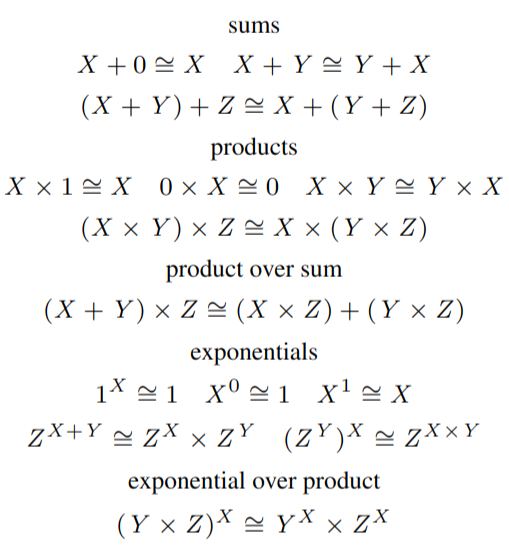
\includegraphics[width=0.4\textwidth]{figs/school-alg}
    \caption{Законы школьной алгебры ностальгии ради~\cite{hinze2010reason}.}
    \label{fig:school-alg}
\end{figure}

\begin{task}
    Покажите, что $(a + b) + c \iso a + (b + c)$.
\end{task}

\begin{task}
    Покажите, что $c^{a + b} \iso c^a\times c^b$.
\end{task}

Интересным наблюдением может быть то, что функции можно использовать как структуры данных, в соответствие с изоморфизмом $c^{a + b} \iso c^a\times c^b$.
Действительно, в таком случае аргумент функции выступает индексом (его кардинальность должна совпадать с размером коллекции).
Это очень важный изоморфизм, мы к нему вернёмся, чтобы проложить путь к tagless-final интерпретаторам и коданным в главе~\ref{sec:wonder-interpreters}.
\begin{minted}{haskell}
    -- ?$a \times a \iso a^2$?
    get :: (a, a) -> (Bool -> a)
    get (x, y) idx = if idx then x else y
    tabulate :: (Bool -> a) -> (a, a)
    tabulate f = (f True, f False)
\end{minted}

\vocab{Каноническим предствлением типа (canonical representaion)} называют сумму произведений типов:
\[
    \sum_{i}\prod_{j} t_{ij}
\]
Каноническое представление является своего рода нормальной формой, в которой можно записывать алгебраические типы (любой алгебраический тип можно по правилам привести к ней).
Легко узнать в нём вид \mintinline{haskell}{data} деклараций в Haskell.
В дальнейшем мы воспользуемся каноническим представлением для обобщённой работы с типами (глава.~\ref{sec:datatype-generic}).

% todo производная

\subsection{Рекурсивные типы} \label{subsec:recursive-types}

В этом разделе мы научимся рассуждать о рекурсивных типах, получать их различные формы.
А так же построим универсальную свёртку.

Рассмотрим классический функциональный список.
Список это либо коллекция из нуля элементов, либо одного, либо двух\ldots
Алгебраически это запишется следующим образом:
\[
    L = 1 + a + a^2 + a^3 + \ldots
\]
Фактически получили тип с бесконечной записью.
Поработаем с ним как с формальным рядом.
Вынесем $a$ за скобки:
\[
    L = 1 + a \times (1 + a + a^2 + \ldots)
\]
Заметим, что выражение в скобках представляет собой список, получим такое рекурсивное уравнение\footnote{Либо можно получить то же самое, заметив, что мы имеем дело с рядом Тейлора \url{https://codewords.recurse.com/issues/three/algebra-and-calculus-of-algebraic-data-types}.}:
\[
    L = 1 + a \times L
\]
Легко видеть, что это на самом деле знакомое нам определение списка из Haskell:
\begin{minted}{haskell}
    data List a = Nil | Cons a (List a)
\end{minted}

\subsubsection{Неподвижная точка функтора} \label{subsubsec:functor-fixpoint}

Получим конечное нерекурсивное представление типа $L$.
Фактически, нам нужно получить тип изоморфный самому себе:
\[
    L \iso 1 + a \times L
\]

Расширим язык типов абстракцией (полиморфизмом) и решим полученное рекурсивное уравнение в стиле $\lambda$-исчисления, с помощью некоторого комбинатора неподвижной точки:
\[
    L = FIX\ap\lambda r\ldotp 1 + a \times r
\]
Перепишем на Haskell:
\begin{minted}{haskell}
    data Fix :: (Type -> Type) -> Type
    data Fix f = In { out :: f (Fix f) }

    data ListShape a r = FNil | FCons a r
    data List' a = Fix (ListShape a)
\end{minted}

\begin{task}
    Какие типы будут у \mintinline{haskell}|In| и \mintinline{haskell}|out|?
\end{task}

Фактически мы разбили рекурсивную структуру данных на две, одна отвечает за рекурсию, вторая --- за форму дерева.
Иначе говоря, вместо того, чтобы сослаться на себя, тип абстрагируется по рекурсивной ссылке, которую ему предоставят снаружи.
Эта техника называется \vocab{открытой рекурсией}.
Так, пользователь может контролировать, рекурсию, чем мы в дальнейшем будем пользоваться.

Можно показать, что \mintinline{haskell}{List a ?$\iso$? List' a}\footnote{Тут используется удобное расширение \href{https://downloads.haskell.org/~ghc/9.0.1/docs/html/users_guide/exts/lambda_case.html}{LambdaCase}, позволяющее не вводить лишние имена.}:
\begin{minted}{haskell}
    to :: List a -> List' a
    to = \case
      Nil -> In FNil
      Cons x xs -> In $ FCons x (to xs)

    from :: List' a -> List a
    from (In shape) = case shape of
      FNil -> Nil
      FCons x xs -> Cons x (from xs)
\end{minted}

Тип формы можно сделать функтором по последнему параметру.
Это позволит нам в дальнейшем заменять вхождения поддеревьев на что-то полезное.
\begin{minted}{haskell}
    instance Functor (ListShape a) where
      fmap :: (rec -> other) -> ListShape a rec -> ListShape a other
      fmap f = \case
        FNil -> FNil
        FCons x xs -> FCons x (f xs)
\end{minted}

Таким образом, мы научились кодировать рекурсивный тип в стиле теории категорий, как неподвижную точку функтора.

\begin{task}
    Выразите следующее дерево как неподвижную точку функтора.
    Объявите инстанс функтора для типа-формы.
    \begin{minted}{haskell}
        data Tree a = Leaf a | Node a (Tree a) (Tree a)
    \end{minted}
\end{task}

\subsubsection{Схемы рекурсии} \label{subsubsec:recursion-schemas}

Подобно тому, как структурное императивное программирование, в сравнении с беспорядочным использованием \texttt{goto}, помогает рассуждать о программах, так \vocab{схемы рекурсии} позволяют алгебраически описывать свойства рекурсивных функций, в отличие от ``неструктурной'' рекурсии\footnote{\url{https://reasonablypolymorphic.com/blog/recursion-schemes/index.html}}~\cite{meijer1991functional, meijer1995bananas}.

Глобальная идея состояла в том, чтобы формулировать требуемые свойства и вычислять нужные программы подобно тому, как математики находят решения дифференциальных уравнений.
Однако, эта идея не нашла нужного развития и применения (однако, владеть алгебраическим подходом в целом полезно~\cite{maguire-algebra}).
Тем не менее это знание, с одной стороны, даёт более глубокое понимание рекурсии, с другой, пригодится нам для рассмотрения и решения главной проблемы этого курса~--- expression problem.

Для начала рассмотрим обобщённую свёртку.
Свёртка в общем смысле позволяет заменить все каждый конструктор данных в дереве на некоторую функцию.
В результате получается вычисление, имеющее доступ ко всему содержимому структуры данных, возвращающее некоторый результат агрегации.
\begin{center}
    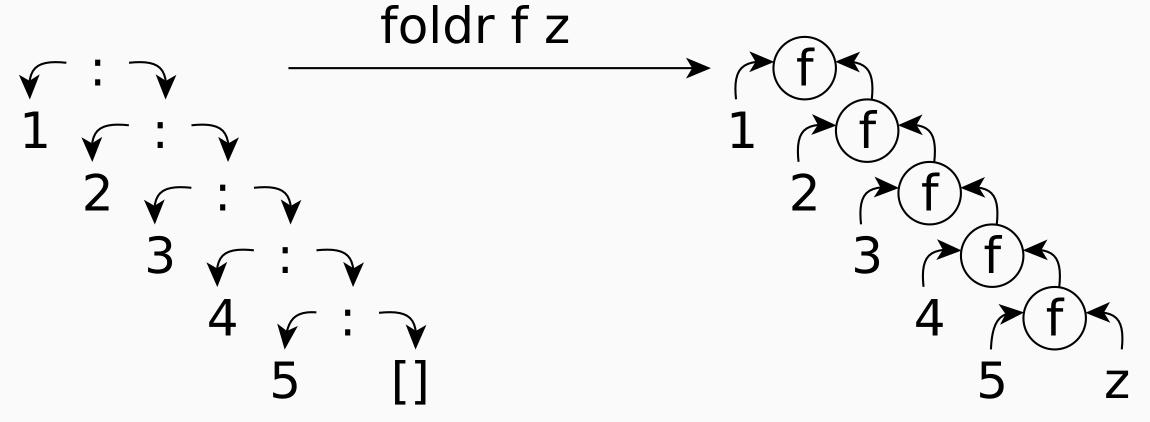
\includegraphics[width=0.5\textwidth]{figs/foldr}
\end{center}

Однако как написать свёртку, работающую для произвольного типа данных?
Функция \texttt{foldr} явно полагается на знание о конструкторах списка --- она принимает ноль-арную функцию \texttt{z} для замены \texttt{[]} и бинарную для \texttt{(:)}.
Нам поможет разделение рекурсивного типа на функтор формы и рекурсивный тип.

Универсальная свёртка называется \vocab{катаморфизмом}.
Катаморфизм сначала рекурсивно сворачивает поддеревья, добираясь к ним с помощью \mintinline{haskell}|fmap|, и оставляет результаты свёртки типа \texttt{a} вместо бывших вхождений поддеревьев.
Получается значение типа \texttt{f a}, где \texttt{f} --- какой-то функтор формы.
Далее применяется функция типа \texttt{f a -> a}, которая определяет, как свернуть один слой рекурсивной структуры, когда поддеревья уже свёрнуты.
\begin{minted}{haskell}
    cata :: Functor f => (f a -> a) -> Fix f -> a
    cata phi = phi . fmap (cata phi) . out
\end{minted}

Например, сумма списка будет выглядеть следующим образом:
\begin{minted}{haskell}
    sum :: List' Int -> Int
    sum = cata \case
      FNil -> 0
      FCons x result -> x + result
\end{minted}

\begin{figure}[h]
    \centering
    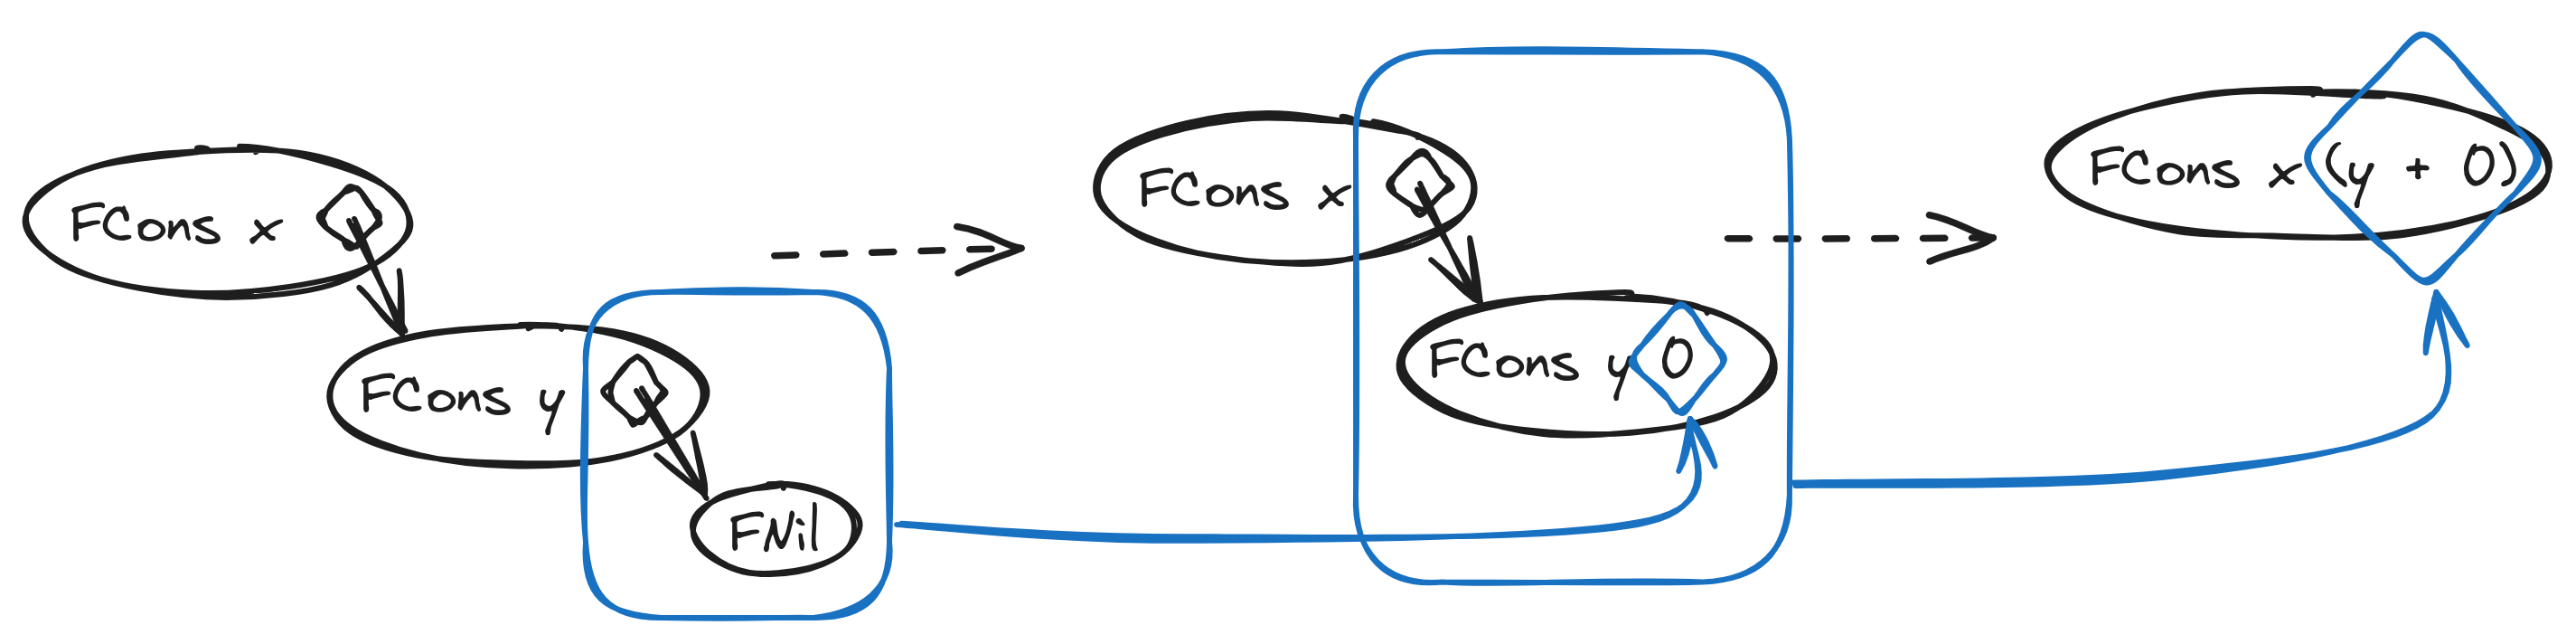
\includegraphics[width=0.8\textwidth]{figs/cataStep.excalidraw}
\end{figure}

\begin{task}
    С помощью какой алгебры можно скопировать структуру данных?
\end{task}

\begin{task}
    С помощью какой алгебры можно распечатать список в строчку?
\end{task}

Функцию \texttt{f a -> a} называют \vocab{f-алгеброй}.
Действительно, если в качестве функтора \texttt{f} взять сигнатуру алгебры, а в качестве \texttt{a} носитель, то f-алгебра будет задавать некоторую интерпретацию сигнатуры:
\begin{minted}{haskell}
    data MonoidSig carrier = Mempty | Mappend carrier carrier

    interpretSig :: MonoidSig Int -> Int
    interpretSig = \case Mempty -> 0; Mappend l r -> l + r
\end{minted}

В противоположность универсальной свёртке, можно построить \vocab{анаморфизм}~---универсальную развёртку.
Здесь f-коалгебра (стрелочка в обратную сторону) показывает, как из некоторого значения-зерна получить один слой структуры данных, где вместо рекурсивных ссылок будут зёрнышки, из которых потом прорастут поддеревья.
Анаморфизм как раз сначала разворачивает один слой, а потом рекурсивно разворачивает все поддеревья:
\begin{minted}{haskell}
    ana :: Functor f => (a -> f a) -> a -> Fix f
    ana psi = In . fmap (ana psi) . psi
\end{minted}

\begin{task}
    Реализуйте анаморфизм, строящий список от $0$ до заданного $n$.
\end{task}

Также вводят \vocab{гиломорфизм (hylomorphism)}, которые позволяют описать произвольное рекурсивное вычисление.
Гиломорфизм задаётся как композиция анаморфизма и катаморфизма.
Сначала анаморфизм строит явное дерево, представляющее собой дерево вызовов некоторой рекурсивной процедуры, затем катаморфизм сворачивает его в результат.
\begin{minted}{haskell}
    hylo :: Functor f => (a -> f a) -> (f b -> b) -> a -> b
    hylo psi phi = cata phi . ana psi
\end{minted}

Например, вычисление факториала может быть реализовано следующим образом:
\begin{minted}{haskell}
    fac n = hylo
      (\n -> if n > 0 then FCons n (n - 1) else FNil)
      (\case FNil -> 1; FCons n acc -> n * acc)
\end{minted}

Можно ввести ещё много различных рекурсивных схем\footnote{\url{https://wiki.haskell.org/Zygohistomorphic_prepromorphisms}} и описать их свойства.
Однако, мы пока остановимся.

% todo где-нибудь сослаться на Пирса

\subsection{Категория алгебр} \label{subsec:cats}

Это факультативный раздел, не являющийся необходимым для понимания курса в дальнейшем.
Однако, полезен для понимания часто употребимой терминологии.

\vocab{Категория} --- это коллекция объектов и коллекция стрелок.
Для каждого объекта $X$ существует тождественная стрелка, а для каждой пары стрелок существует способ получить их композицию: $f : Y \to Z, g : X \to Y \Rightarrow f \circ g : X \to Z$.

Определяют категорию, соответствующую Haskell --- $Hask$.
На самом деле это плохая категория с точки зрения теории, но для наших нестрогих рассуждений подойдёт\footnote{\url{https://math.andrej.com/2016/08/06/hask-is-not-a-category/}}.
Объектами в Hask являются типы языка Haskell, а морфизмами --- термы, задающие функции между соответствующими типами.
Тождественный морфизм --- \mintinline{haskell}|id|, композиция задаётся как \mintinline{haskell}|f . g = \x -> f (g x)|.

\begin{task}
    Как в такой категории представить константы?
\end{task}

\vocab{Функтором} называется отображение между категориями, которое объектам одной категории сопоставляет объекты другой, а стрелкам одной --- стрелки другой.
В Haskell типовые конструкторы задают отображение между объектами, а \mintinline{haskell}|fmap| --- между стрелками.
Функтор должен сохранять тождественный морфизм и композицию.
\begin{figure}[h!]
    \centering
    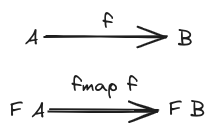
\includegraphics[width=0.25\textwidth]{figs/functor}
\end{figure}

\vocab{Алгеброй} в категории $C$ называется пара из объекта категории $X \in Obj(C)$ и морфизма $\phi : F\ap X \to X$, где $F$ --- функтор.
Сам морфизм $F\ap X \to X$ называют \vocab{f-алгеброй}.
Алгебрами в смысле категорий можно описывать алгебры.
Так, в качестве объекта $X$ берём носитель алгебры.
В качестве функтора $F$ --- сигнатуру алгебры в виде типа-формы.
Тогда морфизмом будет интерпретацией сигнатуры.

\vocab{Морфизмом алгебр} называется такой морфизм между носителями $h : X \to Y$, что следующая диаграмма коммутирует.
Говорят, что \vocab{диаграмма коммутирует}, если все возможные пути по стрелкам в ней равны.
\begin{figure}[h!]
    \centering
    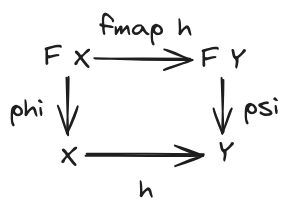
\includegraphics[width=0.3\textwidth]{figs/alg-homomorphism}
\end{figure}

В морфизме алгебр можно обнаружить знакомые черты гомоморфизмов, то есть операций между носителями, которые ``уважают'' операции сигнатуры алгебраической теории.

Алгебры над категорией $C$ образуют \vocab{категорию алгебр}, в которой объектами являются алгебры, а морфизмами --- морфизмы алгебр.

\vocab{Начальным (инициальным) объектом} категории называется объект, из которого в каждый другой объект существует уникальная стрелка.
\vocab{Терминальным (финальным) объектом} категории называется объект, в который из каждого другого объекта категории существует уникальная стрелка.

Инициальный и терминальный объекты категории не обязательно присутствуют в единственном экземпляре.
Но все инициальные объекты изоморфны друг другу, как и все терминальные.

\begin{task}
    Приведите начальный и терминальный объекты категории $Hask$.
\end{task}

Рекурсивный тип --- это тип, значит ему соответствует объект в категории Hask.
$X$ является рекурсивным типом с формой $F$, если имеет место следующий изоморфизм:
\[X \simeq F\ap X\]

Можно заметить, что свидетель изоморфизма справа налево напоминает f-алгебру, а слева направо --- f-коалгебру (всё то же самое, только все стрелки в обратную сторону).
И действительно, подходящий объект $X$ должен быть либо начальным объектом категории алгебр, либо терминальным объектом категории коалгебр (с соответствующими морфизмами).
Первый вариант соответствует конечным структурам данных, второй --- потенциально бесконечным.

Начальным объектом категории алгебр над $Hask$ для функтора $f$ является следующая алгебра: \mintinline{haskell}|(Fix f, In)|\footnote{\url{https://bartoszmilewski.com/2017/02/28/f-algebras/}}\footnote{\url{https://ncatlab.org/nlab/show/catamorphism}}.
Действительно, для каждого типа \texttt{a} и для каждой f-алгебры \texttt{phi} мы можем построить такой морфизм \mintinline{haskell}|cata phi :: Fix f -> a|, что следующая диаграмма будет коммутировать.
\begin{figure}[h!]
    \centering
    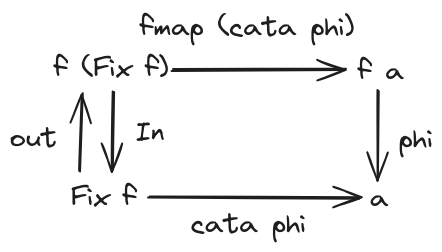
\includegraphics[width=0.4\textwidth]{figs/cata}
\end{figure}

Покажем, что \mintinline{haskell}|(Fix f, In)| является ещё и терминальным объектом (благодаря ленивости Haskell). % todo как тут учитывается ленивость
Аналогично, для каждого объекта \texttt{a} и f-коалгебры \texttt{psi} найдётся морфизм \mintinline{haskell}|ana psi :: a -> Fix f|.
\begin{figure}[h!]
    \centering
    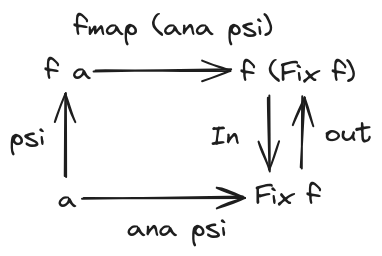
\includegraphics[width=0.35\textwidth]{figs/ana}
\end{figure}

Анаморфизм проясняет интуицию, почему терминальными коалгебрами кодируют потенциально бесконечные структуры данных.
f-коалгебра по некоторому зерну вычисляет следующий слой структуры.
Так, можно слой за слоем лениво вычислять поддеревья, потенциально сколь угодно долго.
